\begin{figure}[H]
    \centering

\begin{tikzpicture}
\pgfplotsset{
    every axis/.style={ymin=0},
    width=0.22\textwidth,
    height=0.25\textheight,
    xtick={1, 2, 3, 4, 5, 6, 7, 8, 9, 10},
    y axis style/.style={
    yticklabel style=#1,
    ylabel style=#1,
    y axis line style=#1,
    ytick style=#1}}
\begin{axis}[ scale only axis, ymin=0, ymax=170, xmin=1,xmax=10, axis y line*=left, xlabel=Number of Cores, ylabel=Execution time (s), y axis style=green!75!black]
    \addplot[smooth, green!75!black, mark=o, draw] 
    coordinates 
    {
        (1,165)
        (2,107)
        (3,88)
        (4,79)
        (5,73)
        (6,71)
        (7,69)
        (8,67)
        (9,66)
        (10,69)
    };
\end{axis}
%
\begin{axis}[ scale only axis, ymin=0, ymax=1800, xmin=1,xmax=10, axis y line*=right, axis x line=none, ylabel=DEC (j), y axis style=blue]%
    \addplot[smooth, blue, mark=x] 
    coordinates 
    {
        (1,549)
        (2,557)
        (3,551)
        (4,556)
        (5,553)
        (6,556)
        (7,556)
        (8,551)
        (9,543)
        (10,538)
    };
\end{axis}
%
\begin{axis}[red, scale only axis, ymin=0, ymax=20, xmin=1,xmax=10, axis y line*=right, axis x line=none, ylabel=DEC per second (w)]%
\pgfplotsset{every outer y axis line/.style={xshift=2cm}, every tick/.style={xshift=2cm}, every y tick label/.style={xshift=2cm} }
    \addplot[smooth, red ,mark=+] 
    coordinates 
    {
        (1,3.34)
        (2,5.17)
        (3,6.26)
        (4,7.03)
        (5,7.58)
        (6,7.77)
        (7,7.99)
        (8,8.04)
        (9,8.07)
        (10,7.78)
    };
\end{axis} 

\end{tikzpicture}
    \caption{The evolution of the DEC (blue), DEC per second (red) and execution time (green) as more cores are allocated to 3DM on DUT 2}
    \label{fig:exp_3_dut_2_3dm_result}
\end{figure}